\begin{frame}[fragile]{DP Haskell Framework}
  \begin{center}
    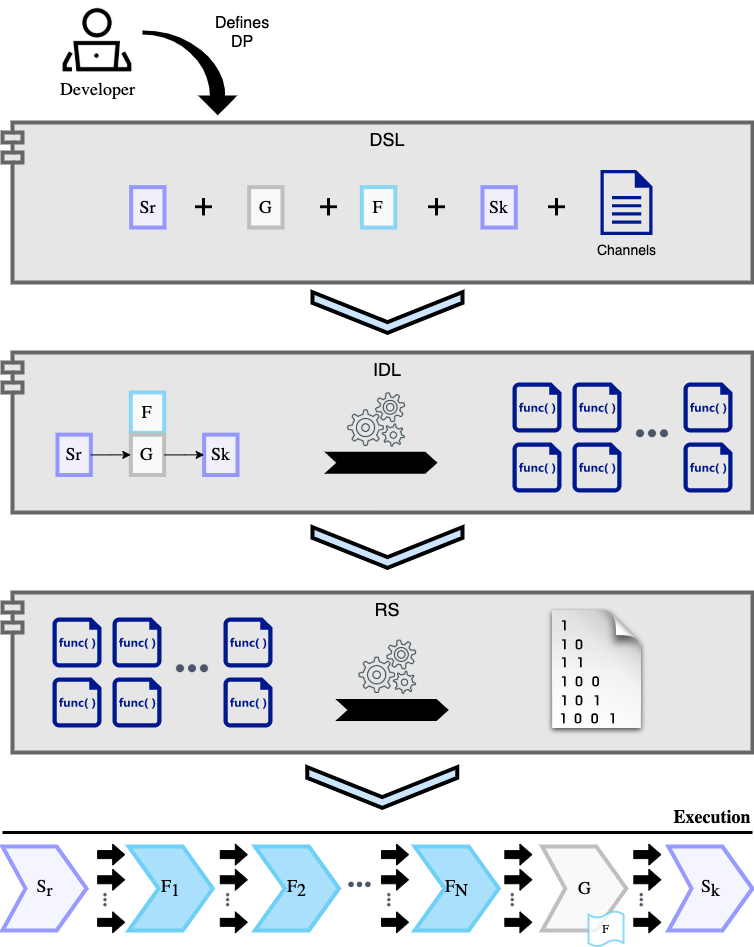
\includegraphics[width = 0.8\textwidth, height = 0.8\textheight]{dpf_haskell_v3}
  \end{center}
\end{frame}

  \begin{frame}[fragile]{DP Haskell Framework}
    \begin{center}
    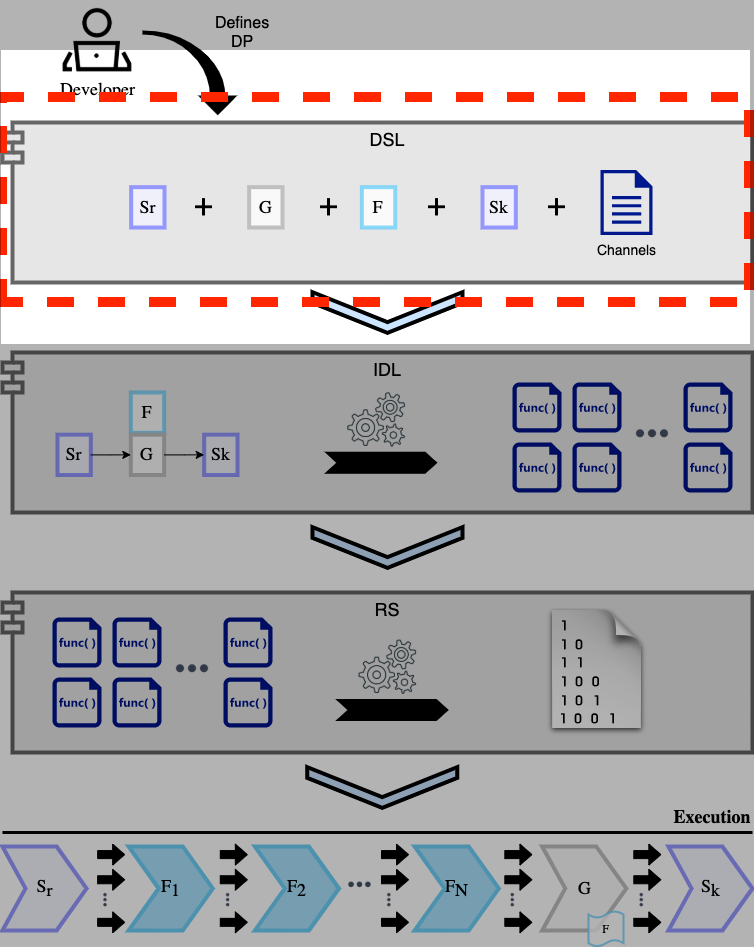
\includegraphics[width = 0.8\textwidth, height = 0.8\textheight]{dpf_haskell_v3-1}
  \end{center}
\end{frame}

\lstset{
  basicstyle=\itshape,
  literate={->}{$\rightarrow$}{2}
}

\begin{frame}[fragile]{DP Haskell Framework}
  \frametitle{DSL Grammar}
  \small
  \begin{equation*}
    \boxed{
     \begin{aligned}
    G_{dsl} = (N, \Sigma, DB, P)
    \end{aligned}
    }
\end{equation*}
\tiny
    \begin{equation*}
        \boxed{
         \begin{aligned}
        N &= \{DP,S_r,S_k,G,F_b,CH,CH_s\},\\
        \Sigma &= \{\text{\mintinline{haskell}{Source}},\text{\mintinline{haskell}{Generator}},\text{\mintinline{haskell}{Sink}},\text{\mintinline{haskell}{FeedbackChannel}},\text{\mintinline{haskell}{Type}},\text{\mintinline{haskell}{Eof}},\text{\mintinline{haskell}{:=>}},\text{\mintinline{haskell}{:<+>}}\},
        \end{aligned}
        }
    \end{equation*}
  \small
  \begin{equation*}
    \boxed{
      \begin{aligned}
    P = \{\\
    DP  &\rightarrow S_r\ \text{\mintinline{haskell}{:=>}}\ G\ \text{\mintinline{haskell}{:=>}}\ S_k\ |\ S_r\ \text{\mintinline{haskell}{:=>}}\ G\ \text{\mintinline{haskell}{:=>}}\ F_b\ \text{\mintinline{haskell}{:=>}}\ S_k,\\
    S_r &\rightarrow \text{\mintinline{haskell}{Source}}\ CH_s,\\
    G   &\rightarrow \text{\mintinline{haskell}{Generator}}\ CH_s,\\
    S_k &\rightarrow \text{\mintinline{haskell}{Sink}},\\
    F_b &\rightarrow \text{\mintinline{haskell}{FeedbackChannel}} CH,\\
    CH_s &\rightarrow \text{\mintinline{haskell}{Channel}}\ CH,\\
    CH &\rightarrow \text{\mintinline{haskell}{Type :<+>}}\ CH\ |\ \text{\mintinline{haskell}{Eof}}\}
  \end{aligned}
  }
  \end{equation*}
\end{frame}

\begin{frame}[fragile]{DP Haskell Framework}
  \begin{itemize}
    \item The specification of \textbf{DP} in the Language is compile time checked (\textit{Type-safe})
  \end{itemize}    
  \begin{exampleblock}{Type Level DSL}
    \begin{minted}[fontsize=\small,breaklines,highlightlines={7-17}]{shell}      
ghci> import DynamicPipeline
ghci> type DPExample = Source (Channel (Int :<+> Eof)) :=> Generator (Channel (Int :<+> Eof)) :=> Sink
type DPExample :: *
type DPExample =
Source (Channel (Int :<+> Eof))
:=> (Generator (Channel (Int :<+> Eof)) :=> Sink)
ghci> :t mkDP @DPExample
mkDP @DPExample
:: forall k (st :: k) filterState filterParam.
    Stage (WriteChannel Int -> DP st ())
    -> GeneratorStage DPExample filterState filterParam st
    -> Stage (ReadChannel Int -> DP st ())
    -> DP st ()    
  \end{minted}
  \end{exampleblock}
\end{frame}

\begin{frame}[fragile]{DP Haskell Framework}
  \begin{center}
    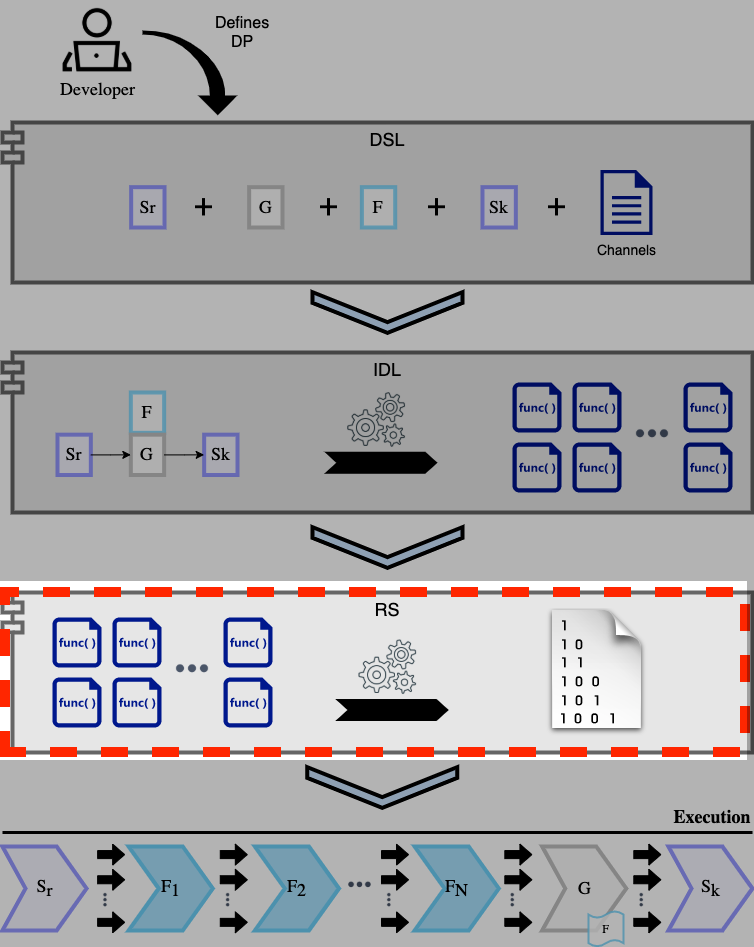
\includegraphics[width = 0.8\textwidth, height = 0.8\textheight]{dpf_haskell_v3-3}
  \end{center}
\end{frame}

\begin{frame}[fragile]{DP Haskell Framework}
  \begin{block}{Runtime System}
    \begin{itemize}
      \item \textbf{DP Monad}:
      \begin{itemize} 
      \item Monad with Existential Type to not escape DP Context. (\textit{Rank-2 Polymorphic type})
      \item Associativity Monad law guarantees execution flow (\mintinline{haskell}{ source >>= generator >>= sink }) 
      \end{itemize}
    \end{itemize}
  \end{block}
  \end{frame}

\begin{frame}[fragile]{DP Haskell Framework}
  \begin{block}{Runtime System}
    \begin{itemize}
      \item \textbf{DP Monad}:
      \begin{itemize} 
      \item Monad with Existential Type to not escape DP Context. (\textit{Rank-2 Polymorphic type})
      \item Associativity Monad law guarantees execution flow (\mintinline{haskell}{ source >>= generator >>= sink }) 
      \end{itemize}
      \item \textbf{Filter / Stage}: 
      \begin{itemize}
        \item Use of \mintinline{haskell}{unfold} to generate dynamic filter computations (\textit{Anamorphism})
        \item Use of \mintinline{haskell}{fold} to reduce results to Sink (\textit{Catamorphism})
      \end{itemize}
    \end{itemize}
  \end{block}
  \end{frame}

\begin{frame}[fragile]{DP Haskell Framework}
  \begin{block}{Runtime System}
    \begin{itemize}
      \item \textbf{DP Monad}:
      \begin{itemize} 
      \item Monad with Existential Type to not escape DP Context. (\textit{Rank-2 Polymorphic type})
      \item Associativity Monad law guarantees execution flow (\mintinline{haskell}{ source >>= generator >>= sink }) 
      \end{itemize}
      \item \textbf{Filter / Stage}: 
      \begin{itemize}
        \item Use of \mintinline{haskell}{unfold} to generate dynamic filter computations (\textit{Anamorphism})
        \item Use of \mintinline{haskell}{fold} to reduce results to Sink (\textit{Catamorphism})
      \end{itemize}
      \item \textbf{Multithreading}: \mintinline{shell}{async} library
    \end{itemize}
  \end{block}
  \end{frame}

\begin{frame}[fragile]{DP Haskell Framework}
\begin{block}{Runtime System}
  \begin{itemize}
    \item \textbf{DP Monad}:
    \begin{itemize} 
    \item Monad with Existential Type to not escape DP Context. (\textit{Rank-2 Polymorphic type})
    \item Associativity Monad law guarantees execution flow (\mintinline{haskell}{ source >>= generator >>= sink }) 
    \end{itemize}
  \item \textbf{Filter / Stage}: 
    \begin{itemize}
      \item Use of \mintinline{haskell}{unfold} to generate dynamic filter computations (\textit{Anamorphism})
      \item Use of \mintinline{haskell}{fold} to reduce results to Sink (\textit{Catamorphism})
    \end{itemize}
    \item \textbf{Multithreading}: \mintinline{shell}{async} library
    \item \textbf{Channels}: \mintinline{shell}{unagi-chan} library
  \end{itemize}
\end{block}
\end{frame}

\begin{frame}[fragile]{DP Haskell Framework}
  \begin{center}
    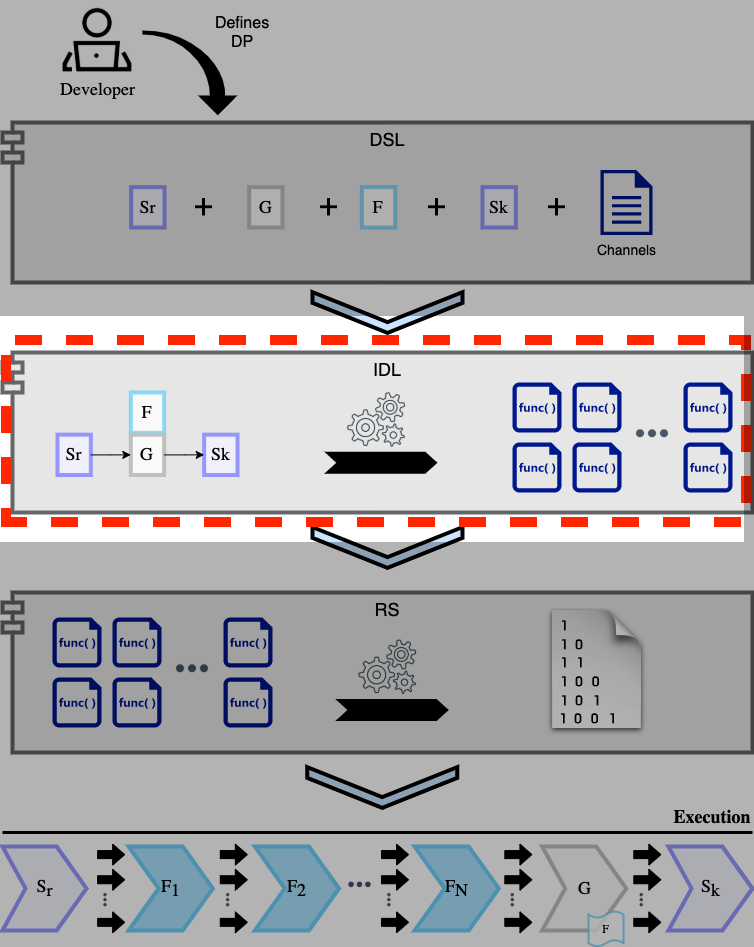
\includegraphics[width = 0.8\textwidth, height = 0.8\textheight]{dpf_haskell_v3-2}
  \end{center}
\end{frame}

\begin{frame}[fragile]{DP Haskell Framework}
  \begin{block}{IDL}
    \begin{minted}[fontsize=\small,breaklines]{shell}      
ghci> type DPExample = Source (Channel (Int :<+> Eof)) :=> Generator (Channel (Int :<+> Eof)) :=> Sink
type DPExample :: *
type DPExample =
Source (Channel (Int :<+> Eof))
:=> (Generator (Channel (Int :<+> Eof)) :=> Sink)
  \end{minted}
\end{block}
\end{frame}

\begin{frame}[fragile]{DP Haskell Framework}
  \begin{block}{IDL}
    \begin{minted}[fontsize=\small,breaklines,highlightlines={7-11}]{shell}      
ghci> type DPExample = Source (Channel (Int :<+> Eof)) :=> Generator (Channel (Int :<+> Eof)) :=> Sink
type DPExample :: *
type DPExample =
Source (Channel (Int :<+> Eof))
:=> (Generator (Channel (Int :<+> Eof)) :=> Sink)
      
ghci> :t withSource @DPExample
withSource @DPExample
:: forall k (st :: k).
    (WriteChannel Int -> DP st ())
    -> Stage (WriteChannel Int -> DP st ())
  \end{minted}
\end{block}
\end{frame}

\begin{frame}[fragile]{DP Haskell Framework}
  \begin{block}{IDL}
    \begin{minted}[fontsize=\small,breaklines,highlightlines={7-9}]{shell}      
ghci> :t withSource @DPExample
withSource @DPExample
:: forall k (st :: k).
    (WriteChannel Int -> DP st ())
    -> Stage (WriteChannel Int -> DP st ())
    
ghci> let source' = withSource @DPExample  $ \wc -> unfoldT ([1..10] <> [1..10]) wc identity
ghci> :t source'
source' :: forall k (st :: k). Stage (WriteChannel Int -> DP st ())
  \end{minted}
\end{block}
\end{frame}

\begin{frame}[fragile]{DP Haskell Framework}
  \begin{block}{IDL}
    \begin{minted}[fontsize=\small,breaklines,highlightlines={2-8}]{shell}      
ghci> :t withGenerator @DPExample
withGenerator @DPExample
:: forall k filter (st :: k).
    (filter -> ReadChannel Int -> WriteChannel Int -> DP st ())
    -> Stage
        (filter -> ReadChannel Int -> WriteChannel Int -> DP st ())    
  \end{minted}
\end{block}
\end{frame}

\begin{frame}[fragile]{DP Haskell Framework}
  \begin{block}{IDL}
    \begin{minted}[fontsize=\small,breaklines,highlightlines={2-8}]{shell}      
ghci> :t withGenerator @DPExample
withGenerator @DPExample
:: forall k filter (st :: k).
    (filter -> ReadChannel Int -> WriteChannel Int -> DP st ())
    -> Stage
        (filter -> ReadChannel Int -> WriteChannel Int -> DP st ())    
  \end{minted}
\end{block}
\begin{block}{Techniques}
  \begin{itemize}
    \item First Class Families
    \item Type-level Defunctionalization 
    \item Defunctionalization
    \item Associated Type Families
  \end{itemize}
\end{block}
\end{frame}

\begin{frame}[fragile]{DP Haskell Framework}
  \begin{block}{}
    Library released on Hackage \\
    https://hackage.haskell.org/package/dynamic-pipeline
    \begin{center}
      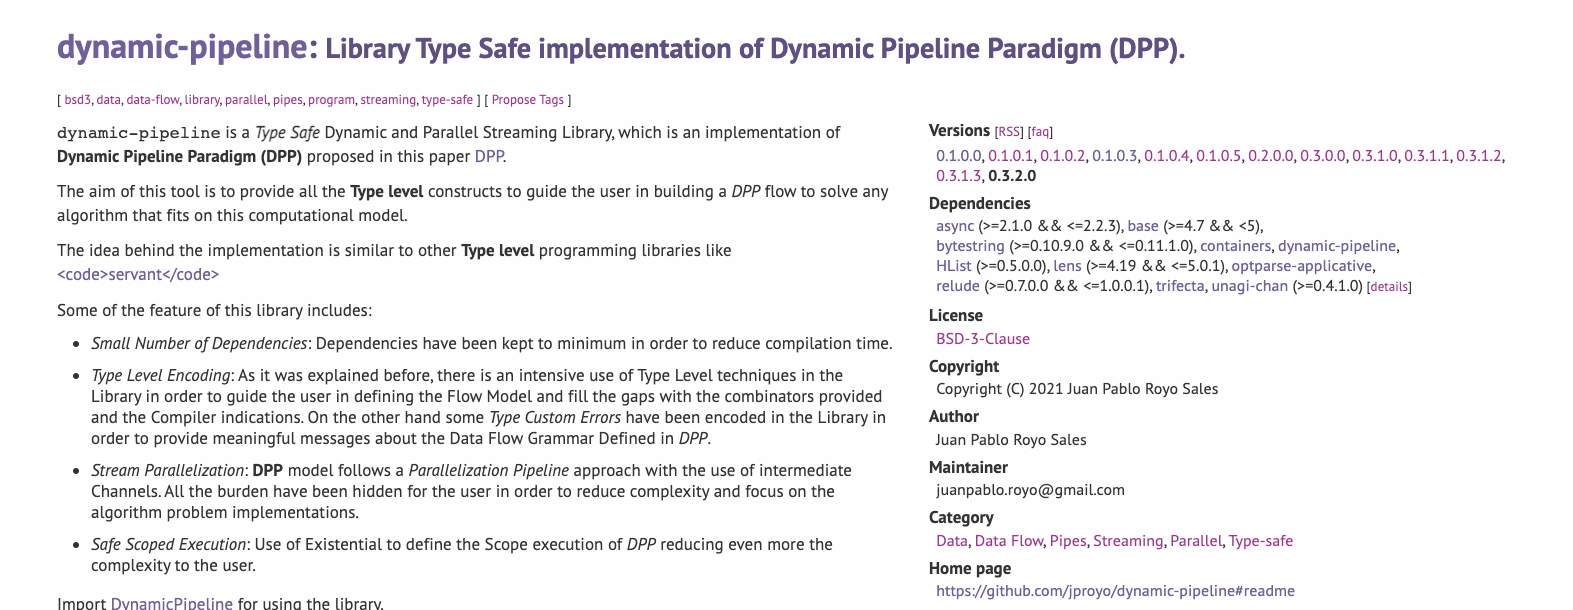
\includegraphics[width = 0.9\textwidth, height = 0.6\textheight]{dp-fw-hs}
    \end{center}  
  \end{block}
\end{frame}
